\documentclass{llncs}

\usepackage{graphicx}
\usepackage{makeidx}
\usepackage{todonotes}
\usepackage{amsmath}
\usepackage{algorithmic}
\usepackage[margin=1in]{geometry}

\begin{document}

\mainmatter
\title{Modeling Heterogeneous Traffic Performance \\ with the 802.11 DCF Access Scheme}
\author{Tamir Husain and Christopher A. Wood}
\maketitle

\begin{abstract}
%\boldmath
% TODO
\end{abstract}

\section{Introduction}
Wireless networks have become pervasive in modern computer and communication systems. The widespread adoption of mobile and personal computing devices, such as smartphones and tablets, continues to drive commercial investment in high performance wireless networking technologies. Concurrently, the type of traffic traversing these networks has also evolved -- divergently -- an increasing rate. Every kind of information from textual data to video stream segments now traverses wireless networks. Society's dependence on WLAN technologies such as the 802.11 protocol suites have cultivated a massive amount of analytical and experimental research studying their performance. 

To date, a major portion of this research has focused on the 802.11 random access control protocol -- the distributed control function (DCF). This work was pioneered by Bianchi's original Markov model for the DCF function \cite{bianchi1996performance}, which stimulated several advancements to his simplistic model \cite{bianchi1998ieee} and numerous applications in the field \cite{crow1996performance,chhaya1997performance}. Many of these models and empirical studies represent a network of nodes by a single collision parameter. In particular, there is a lack of work combining these models together beyond a single parameter. Furthermore, many of these works study the performance of the DCF function (with respect to individual and average system throughput) for single types of traffic. True multi-node models that study the interaction of different traffic models have not been studied.

The goal of this work is to determine if the random behavior of the DCF protocol is best suited for all types of traffic, or if the DCF should in some way be tailored to the \emph{type} of underlying traffic being served by the DCF access scheme. To this end, we first present a series of extensions to Bianchi's original DCF Markov model to emulate arbitrary types of traffic. In particular, we provide extensions to support arbitrary packet length and variable packet inter-arrival time. We then instantiate individual instances of these Markov models that emulate the behavior of the DCF access scheme by tailoring each of these parameters, e.g., packet length and interarrival time, using realistic values drawn from these types of modern application traffic. Following this, we combine these model instances to study the performance of the DCF function with respect to heterogeneous traffic in a true multi-node system. 

Our experimental results seem to provide evidence that the deterministic nature of multimedia (e.g., store-and-forward) traffic streams obtain higher performance than more nondeteministic (elastic) traffic. Furthermore, our results show that large interarrival time between traffic packets benefits the coexistence of heterogeneous traffic streams. 

\section{Related Work}
% \cite{dcf}
% \cite{dcf-nonsaturated}
% TODO

%%% simulation papers
% bianchi1998ieee
% bianchi1996performance
% crow1996performance
% chhaya1997performance

\section{Heterogeneous Traffic Models}
Today's computer and communication networks are being used to transfer increasingly heterogeneous traffic between parties. In particular, file downloads, standard web browsing, video streaming, and client-server video game traffic are four very common types of traffic that dominate the Internet traffic today. In this section, we describe the characteristics of each of these traffic types. We use a variety of parameters to describe these types of traffic. Specifically, we focus on packet size, interrival time, traffic saturation, and burstiness. \\

\noindent
\textbf{File Download Traffic:} File downloads are elastic, meaning that they must be reliable but are also tolerant to random delays. Applications that \emph{generate} file download traffic usually do so with long bursts of packet arrivals and long interarrival times \cite{kumar2004communication}. File downloads are sufficiently random that we do not consider a fixed distribution for any parameters. Rather, we choose these at random by our own free will. \\

\noindent
\textbf{Web Browsing Traffic:} Web browsing traffic is quite diverse in packet size, interrarival time, and burstiness. Mah \cite{mah1997empirical} studied various web browsing traces to develop statistics for these characteristics. In particular, it was found that these characteristics, such as content request and reply lengths (packet size) follow a Zipf disribution (see Figures \ref{fig:histogram1} and \ref{fig:histogram2}).For simplicity, we assume that web browsing traffic has random packet sizes sample from a Zipf distribution, deterministic interarrival time, and probabilistic packet arrival in the buffer. This enables us to use a slightly modified version of the nonsaturated DCF model (described in Section \ref{sec:nonsaturated}) to study this traffic. \\

\begin{figure*}
\begin{center}
\begin{tabular}{cc}
\includegraphics[scale=0.3]{histogram1.png} & \includegraphics[scale=0.3]{histogram2.png} \\
\multicolumn{2}{c}{Distribution of web traffic request and reply sizes, respectively \cite{mah1997empirical}.}
\end{tabular}
\end{center}
\end{figure*}

\noindent
\textbf{Video Streaming Traffic:} Video streaming traffic as described in \cite{badia2010markov} is composed of two types of packets -- I and D packets -- each of which are tightly correlated and with different characteristics. Video segments are sent in sets of I and D packets, wherein multiple small D packets carrying video data are dependent on a single I packet with metadata necessary to decode the video stream. The length of each I and D packet is correlated to past packet lengths. For example, let $\lambda_j(t|s)$ denote the probability that a packet of type $j \in \{I ,D \}$ is $t$ time slots long given that the previous packet of type $j$ was $s$ packets long. The size of both I and D packets are bounded within a finite range so as to make the analytical model tractable. 

In this work we consider a more specific type of multimedia encoding scheme, namely, MPEG. MPEG video traffic streams consist of I, P, and B packets \cite{sony-demo}. In this case, a single I frame is transmitted, is an intraframe and is heavily coded (thus, larger) to ensure it can be correctly decoded by all receivers. P frames follow the I frame, and are used to transmit actual multimedia data. These rely on the previous I frame and P frames to be decoded correctly. B frames -- bidirectional frames -- are transmitted in between I and P frames and naturally serve to relay information in both directions. 

\begin{figure*}
\begin{center}
\includegraphics[scale=0.35]{frame.png}
\caption{Distribution of multimedia frame sizes \cite{sony-demo}.}
\label{fig:frame}
\end{center}
\end{figure*}

\begin{figure*}
\begin{center}
\includegraphics[scale=0.35]{gop.png}
\caption{Distribution of GoP sizes in multimedia traffic \cite{sony-demo}.}
\label{fig:gop}
\end{center}
\end{figure*}

To further understand the differences between these types of traffic, we used our simulator to generate system state transition traces in the context of a simulator. The results of these traces are shown in Figure \ref{fig:traces}. Note that the superposition all traces, shown in the bottom Figure, is the object of study in this work. Namely, we seek to understand the behavior of the DCF as it serves packets generated from sources of heterogeneous traffic.

\begin{figure*}
\begin{tabular}{cc}
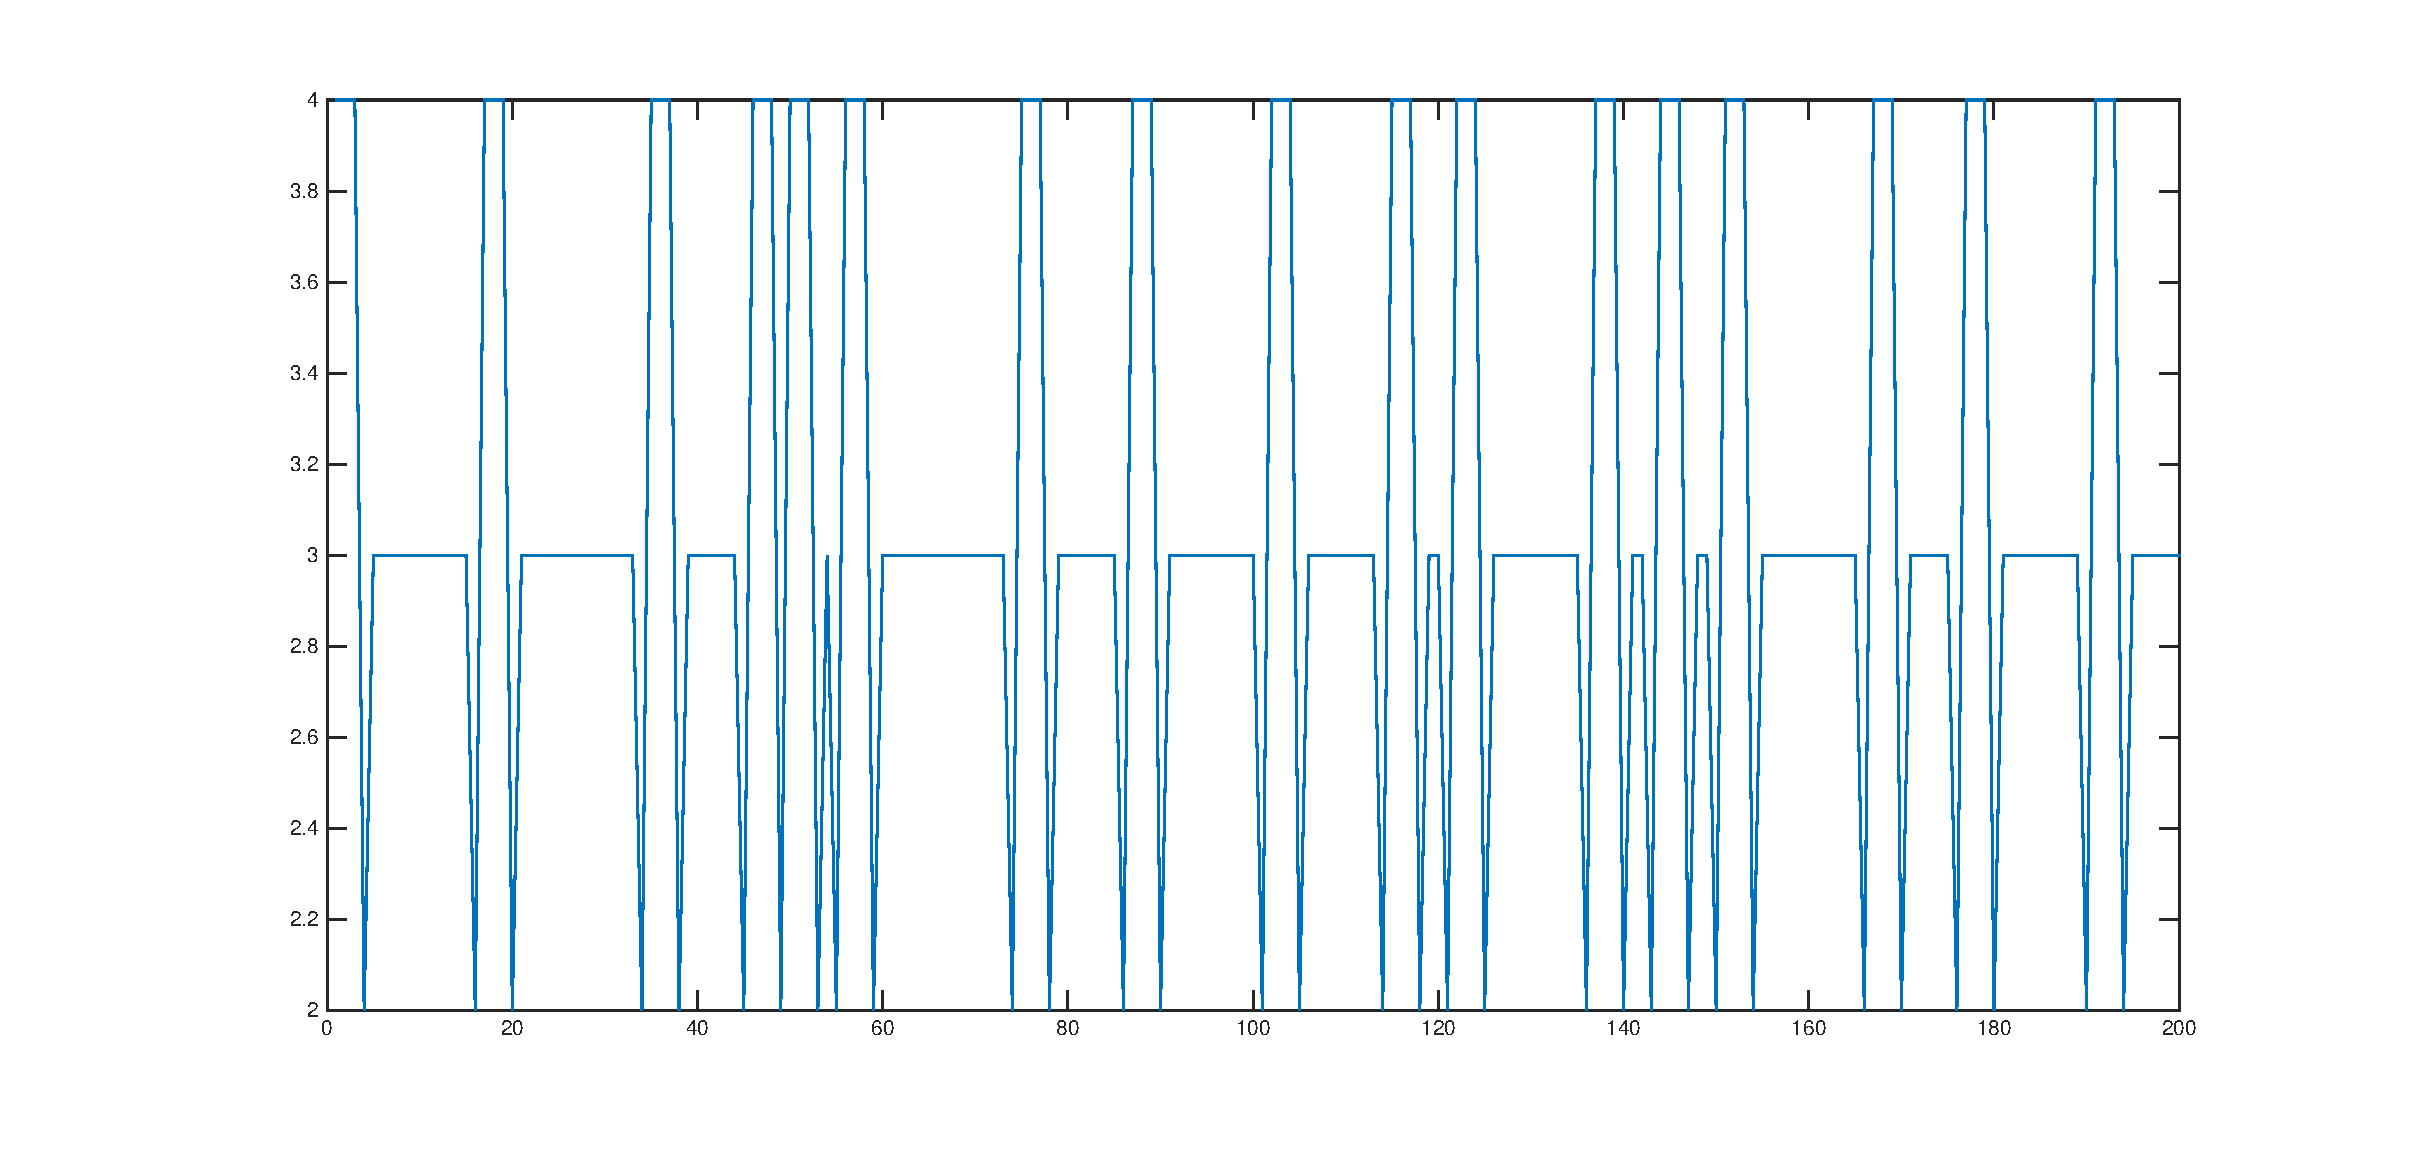
\includegraphics[width=\textwidth,height=100px]{../../src/results/browse_time.eps} \\
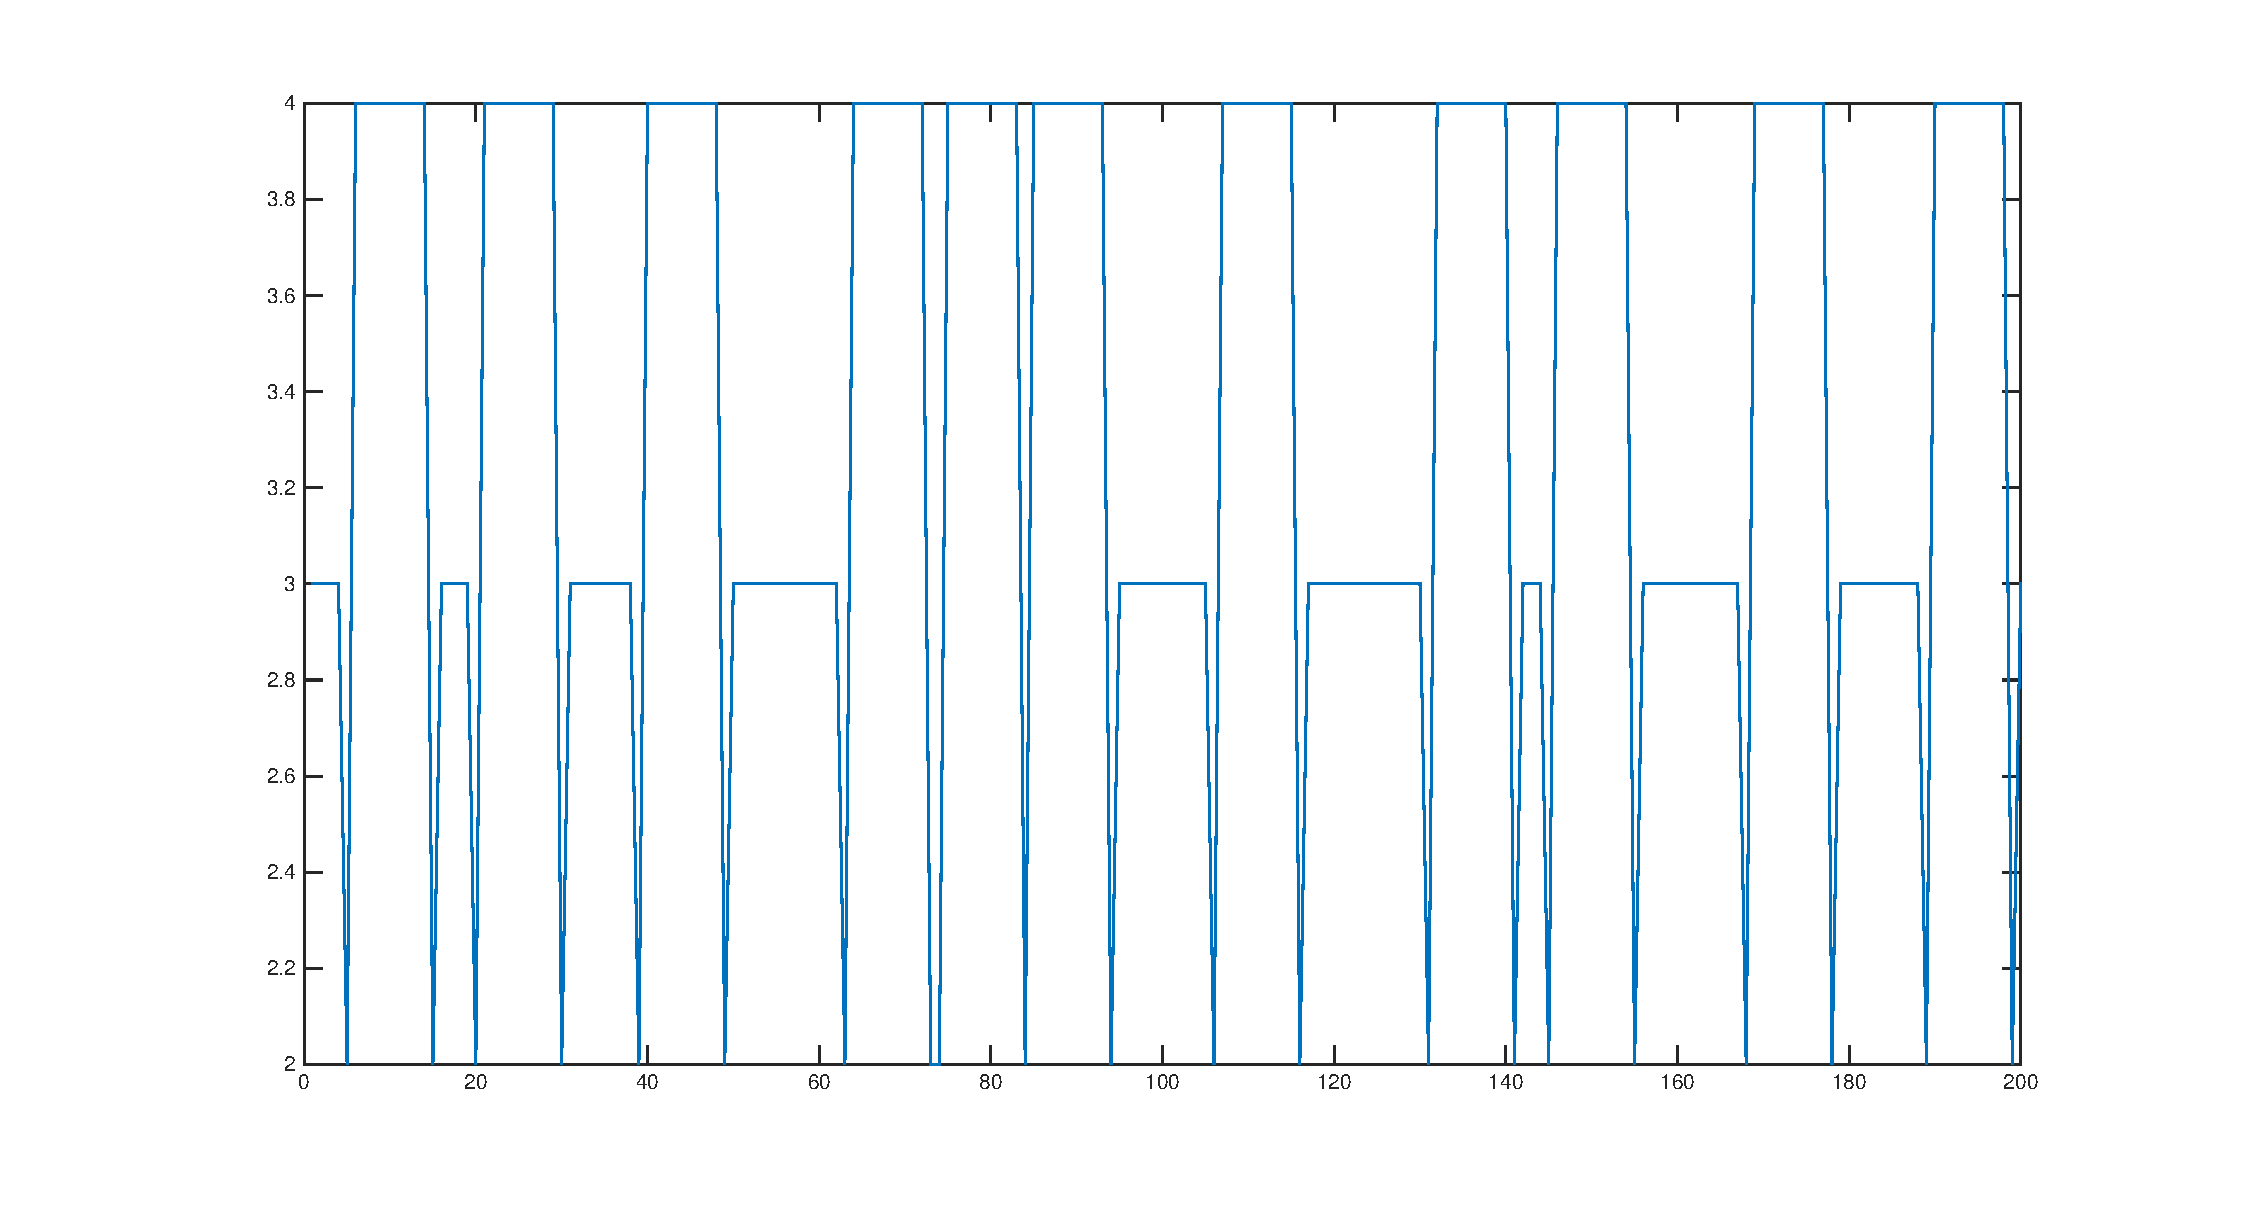
\includegraphics[width=\textwidth,height=100px]{../../src/results/file_time.eps} \\
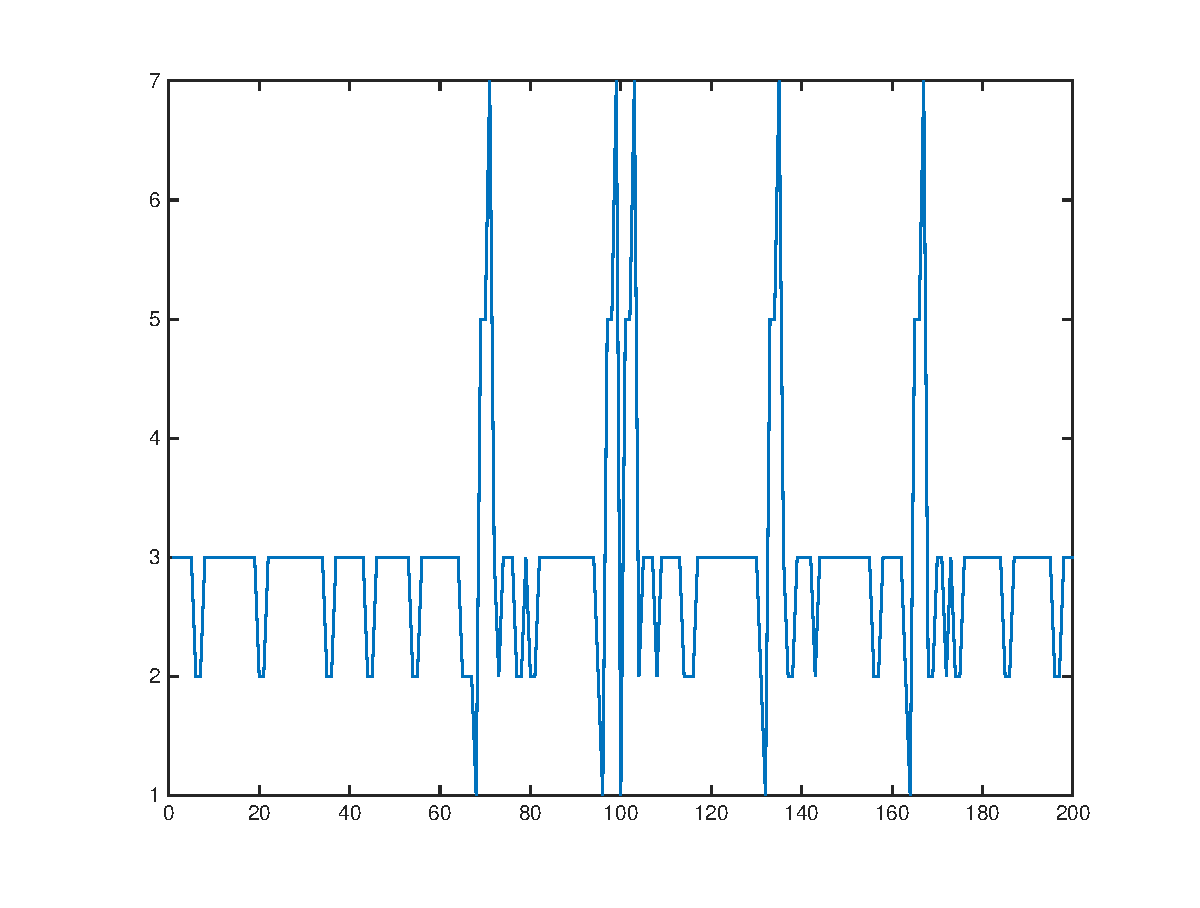
\includegraphics[width=\textwidth,height=100px]{../../src/results/video_time.eps} \\
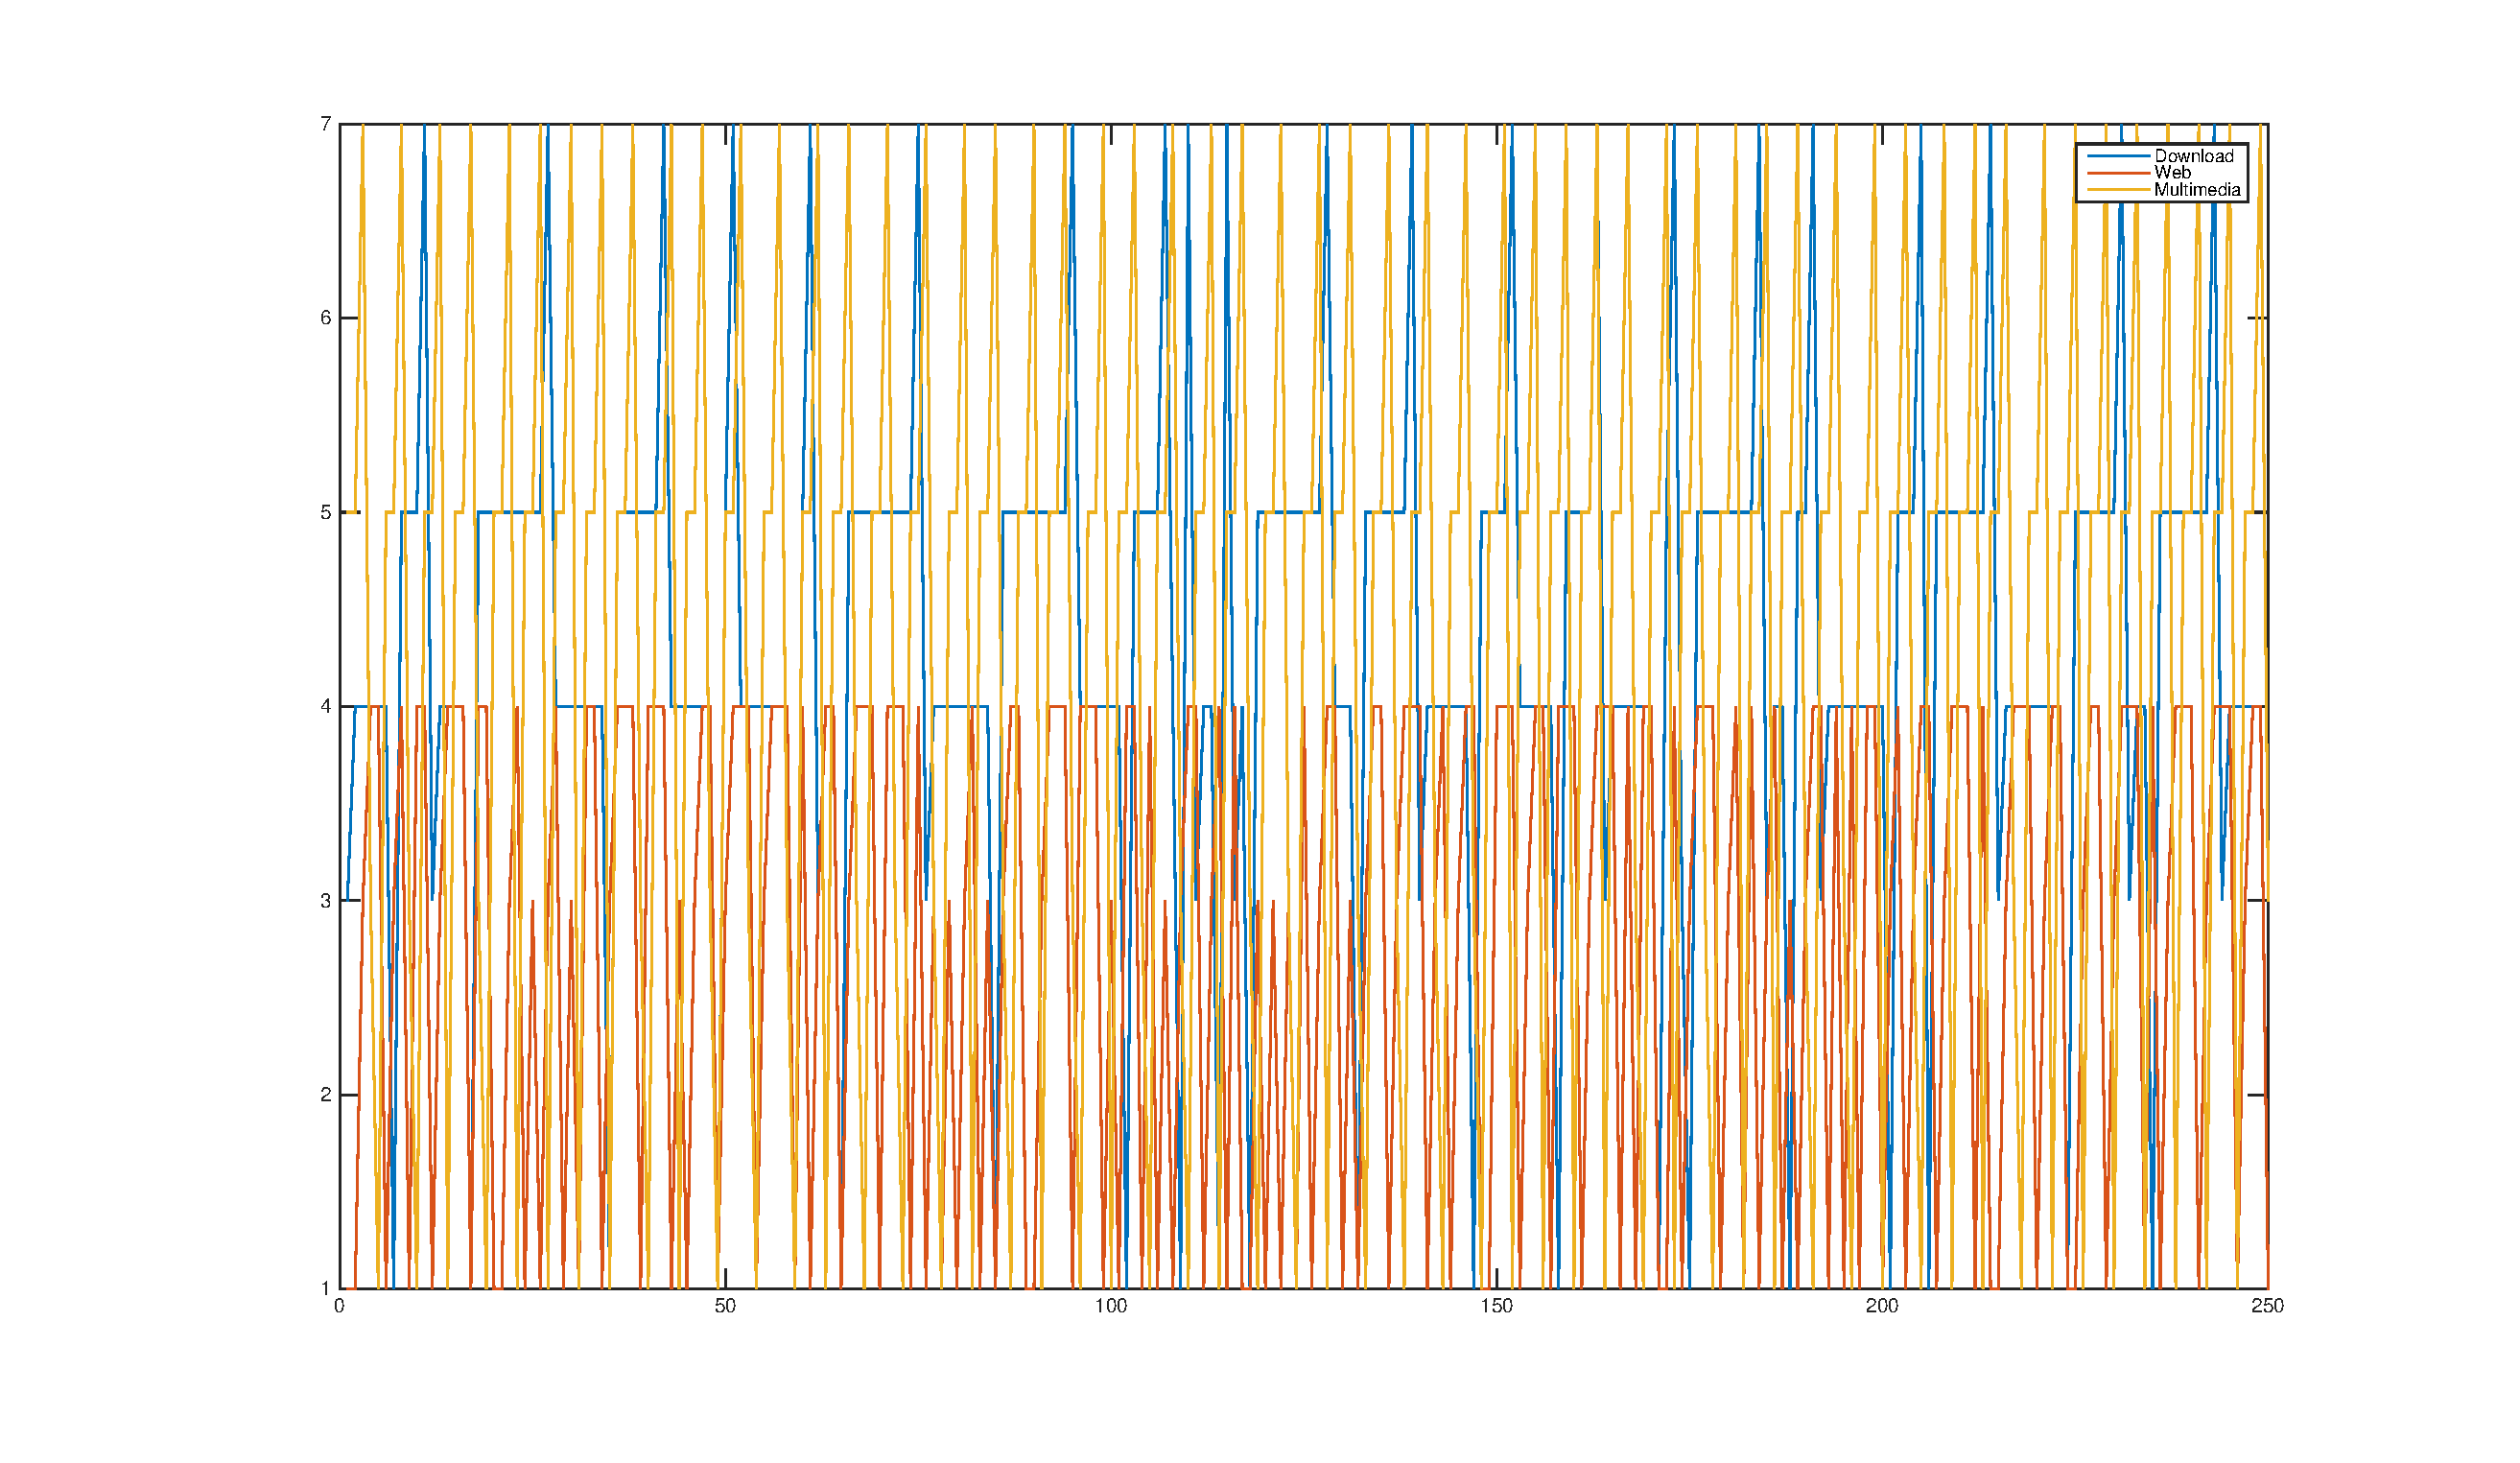
\includegraphics[width=\textwidth,height=100px]{../../src/results/all.eps} \\
\end{tabular}
\caption{Individual system transition traces for (1) web browsing, (2) file download, and (3) video streaming traffic. The bottom trace shows the superposition of all the above traces. The $x$ axis is the discrete time in the system, and the $y$ axis is the state. For completeness, state $5$ is interarrival, $4$ is the packet size calculation, $3$ is a waiting state (e.g., backoff, postbackoff), $2$ is a failure transmission, and $1$ is a successful transmission.}
\label{fig:traces}
\end{figure*}

We will use the characteristics of each of these models to tune our Markov models in the experimental section of this report. 

\section{The 802.11 Distributed Control Function}
The 802.11 DCF \cite{ieee1997wireless} is at the core of this work. It is a simplistic random access scheme based on the carrier sense multiple access with collision avoidance (CSMA/CA) protocol. Failed packets are retried according to a binary exponential backoff rule. At each packet transmission, the backoff is uniformly in the range ($0, w-1$), where $w$ is the length of the ``contention window'' and is directly dependent on the number of failed attempts for the packet thus far. The window $w$ is set to $W_{min}$ to begin, and upon every failure, the backoff counter is doubled. At stage $i$, the backoff timer is $2^iW_{min}$. The maximum backoff is bounded by $W_{max} = 2^mW_{min}$. Selections of $W_{min}$ and $W_{max}$ are dependent upon the physical layer specifications in the 802.11 standard \cite{ieee1997wireless,dcf}. For example, frequency hopping spread spectrum calls for $W_{min} = 16$ and $W_{max} = 1024$ ($m = 6$). 

\section{Incremental Markov Models for Heterogeneous Traffic}
In this section we describe the necessary evolutions of Bianchi's original Markov model to support parameterized packet length, interarrival time, and buffer saturation.

\subsection{Original DCF Model}
A simple Markov model for the 802.11 DCF function was proposed in the seminal work by Bianchi \cite{dcf}. The system state is described by two discrete-time stochastic processes $b(t)$ and $s(t)$: $b(t)$ represents the backoff \emph{time counter} and $s(t)$ represents the backoff \emph{stage} for a given station or node, each of which is advanced at each time step (i.e., from $t$ to $t + 1$). Each node is equipped with a \emph{saturated} buffer of packets to transmit; there is never a case where a node has to wait for a packet to arrive in the buffer before attempting a transmission. Also, instead of modeling multiple nodes simultaneously to accurately assess the probability of collision, this model assumes a constant probability of collision $p$ -- the conditional collision probability -- at each time slot. In the real world, this probability is a function of the network and environmental interferences, e.g., shadowing, fading, etc. However, by making this a constant and therefore independent from other nodes, the model simplifies to capturing the dynamics of the bidimensional process $\{ b(t), s(t) \}$ as a discrete-time Markov chain, shown in Figure \ref{fig:dcf_model}. 

The only non-null transition probabilities in this Markov chain are given below:

\begin{center}
\begin{math}
\boxed{
\begin{array}{lll}
\Pr[i,k | i, k + 1] = 1, & k \in [0, W_i - 2], & i \in [0,m] \\
\Pr[0,k | i, 0] = (1-p)/W_0, & k \in [0, W_0 - 1], & i \in [0,m] \\
\Pr[i,k | i-1, k] = p/W_i, & k \in [0, W_i - 1], & i \in [1,m] \\
\Pr[m,k | m,0] = p/W_m, & k \in [0, W_m - 1] & ~
\end{array}
}
\end{math}
\end{center}

\begin{figure*}
\begin{center}
\includegraphics[scale=0.35]{../../sketches/dcf_model.pdf}
\caption{The original saturated DCF Markov model \cite{dcf}.}
\label{fig:dcf_model}
\end{center}
\end{figure*}

\subsection{Limited and Diverse Traffic} \label{sec:nonsaturated}
While accurate, the original DCF model is constrained in that it assumes homogeneous traffic and a saturated stream of packets for transmission. Malone et al. \cite{dcf-nonsaturated} presented a modified version of Bianchi's model that captures non-saturated traffic loads. The essential idea behind their variant is that there exists a constant packet arrival probability $q$ at each time slot, much like there exists a constant collision probability $p$. If a node successfully transmits a packet and the buffer is not-empty, the state of the system proceeds as normal. Conversely, if a packet is not ready for transmission, then the chain enters a stage known as ``postbackoff,'' denoted $(0,k)_e$ for $k \in [0, W_0-1]$. A node may remain in this set of states indefinitely until a packet arrives and the channel is idle.

To capture the mechanics of the DCF function in this condition, the postbackoff set of stages are nearly indentical to backoff stage $i = 0$. If a packet arrives at any time when the system is in a postbackoff state, it immediately transitions into the backoff stage $i = 0$, with a decremented backoff timer. However, if the postbackoff timer reaches $0$, where the postbackoff is said to be complete, the node will stay in this state until a packet arrives with probability $q$. Once a packet arrives in state $(0, 0)_e$ with probability $q$, there are three possible outcomes: (1) the packet is transmitted successfully, a collision occurs with probability $p$, or the medium (channel) is sensed as busy with probability $1 - P_{idle} = p$. 

With the addition of the postbackoff states $S'$, the Markov chain itself is now a multidimensional process $\{b(t), s(t), S' \}$. The new state transition probabilities needed to capture the transitions between these multiple dimensions are below.

\begin{center}
\begin{math}
\boxed{
\begin{array}{lll}
\Pr[(i,k-1) | (i, k)] = 1 & k \in [1, W_i-1] & i \in [1,m] \\
\Pr[(0,k-1)_e | (0, k)_e] = 1-q & k \in [1, W_i-1] & i \in [1,m] \\
\Pr[(0,k-1) | (0, k)_e] = q & k \in [1, W_i-1] & i \in [1,m] \\
\Pr[(0,k)_e | (i, 0)] = \frac{(1-p)(1-q)}{W_0} & k \geq 0 & i \in [0,m] \\
\Pr[(0,k) | (i, 0)] = \frac{(1-p)q}{W_0} & k \geq 0 & i \in [0,m] \\
\Pr[(\max\{(i+1,m\}, k) | (i, 0)] = \frac{p}{W_{\max\{i+1,m\}}} & k \geq 0 & i \in [0,m] \\
\Pr[(0,0)_e | (0, 0)_e] = 1 - q + \frac{qP_{idle}(1 - p)}{W_0} & ~ \\
\Pr[(0,k)_e | (0, 0)_e] = \frac{qP_{idle}(1 - p)}{W_0} & k > 0 \\
\Pr[(1,k) | (0, 0)_e] = \frac{qP_{idle}p}{W_1} & k \geq 0 \\
\Pr[(0,k) | (0, 0)_e] = \frac{q(1 - P_{idle})}{W_0} & k \geq 0 \\
\end{array}
}
\end{math}
\end{center}

\begin{figure*}
\begin{center}
\includegraphics[scale=0.35]{../../sketches/dcf_model_nonsaturated.pdf}
\caption{The modified DCF Markov model that captures non-saturated traffic \cite{dcf-unsaturated}.}
\label{fig:dcf_model_nonsaturated}
\end{center}
\end{figure*}

Malone et al. \cite{dcf-nonsaturated} exploited the inclusion of this postbackoff state and the fixed arrival probability constant to study the performance of the DCF while transferring packets from unsaturated heterogeneous traffic, e.g., file downloads, web traffic, etc. However, their analysis was limited in scope, since heterogeneous traffic types were parameterized only by $p$ and $q$.

\subsection{Adding Variable Length Frame Payloads}
Despite the flexibilty in the previous model, it is still limited with respect to packet size. In particular, the model assumes that each packet has an equally sized payload. This is not true, especially for video traffic \cite{badia2010markov}, which typically consists of two types of packets of distinctly different sizes: $d$ packets are small video frame/segment packets that carry information needed to render a piece of video data, and $i$ packets are large ``metadata'' packets that contain information necessary to decode $d$ packets. Multiple $d$ packets are often tied to a single $i$ packet in such a way that if the $i$ packet is lost, none of its children $d$ packets can be decoded correctly. Consequently, we need to be able to model packets of different sizes. 

To do this, we consider a range of possible packet sizes, e.g., $[1,l]$, where $l$ is the maximum packet payload size. In this context, the packet size corresponds to \emph{how many} discrete time slots are needed to transfer the content over the channel. In the previously two discussed models, the packet size was assumed to be $1$ since they were assumed to be transferred in a single time step. Since we may want to support both deterministic and arbitrary packet sizes, drawn from a specific distribution, we use what we call size chain blackboxes to capture this type of variability. Figure \ref{fig:size_chain} shows a sample size chain blackbox for the range of values $[1,4]$. There are $l$ ($l = 4$) transitions into the blackbox, and each transition $l'$ is to a chain of length $l'$. 

\begin{figure}
\begin{center}
\includegraphics[scale=0.35]{../../sketches/size_chain_old.pdf}
\caption{A blackbox Markov chain that captures bounded variabilities in a particular parameter, such as packet length or packet interarrival time.}
\label{fig:size_chain}
\end{center}
\end{figure}

To show how this chain would be used, assume that the size chain blackbox represents the size of a particulr packet. Further, assume that the packet size is a discrete random variable ranging from 1 to 4 with uniform distribution. The probability of transferring to any chain within the blackbox from the entry state is $(1/4)$. If the transition was to the last chain of length $l = 4$, then the state would appear to ``loop'' in place for 4 time steps before exiting the blackbox. Conversely, if the transition was to the first chain of length $l = 1$, then the state would only loop once before exiting. Although these states are costly from the persepctive of space, this type of construction enables us to model such discrete random variables with any distribution within our Markov chain. 

The first application of these size chain blackboxes are to extend the previously discusssed nonsaturated model to support variable packet sizes. Specifically, the number of time steps needed to transfer a packet and detect collision is now a bounded discrete random variable. This means that once a packet has begin transmitting it enters a size chain blackbox before either (a) detecting collision or (b) completing successfully. It is important to note that for packets of length $l > 1$, the probability of a collision is no longer $q$. Rather, a collision occurs if there is a collision in \emph{any} time slot during which the packet was being transmitted. This means that the probability of collision for a packet of length $l$ is $1 - (1 - p)^l$. 

The new states required to model the size chain blackboxes are tuples of the form $(i, l, l')$, where $i$ is the backoff stage and $l$ is the packet length, and $l'$ is the \emph{state} within the size chain of length $l$. For example, if the state transitions into a size chain of length $l = 4$ from state $(i, 0)$, then the following series of transitions would occur: 
\begin{align*}
(i, 4, 4) & \to (i, 4, 3) \\
& \to (i, 4, 2) \\
& \to (i, 4, 1)
\end{align*}

To model this behavior, which is visually shown in Figure \ref{fig:dcf_model_unsaturated_varpktsize}, the following new state transition probabilities are included into the model:

\begin{center}
\begin{math}
\boxed{
\begin{array}{lll}
\Pr[(i,l,l'-1) | (i,l,l')] = 1 & l' \leq l & l' \geq 0 \\
\Pr[(i+1,k) | (i,l,0)] = \frac{1 - (1 - p)^l}{W_{i+1}} & ~ & k \in (0, W_{i+1} - 1) \\
\Pr[(0,k) | (i,l,0)] = \frac{(1 - q)(1 - p)^l}{W_0} & ~ & k \in (0, W_{0} - 1) \\
\Pr[(0,k)_e | (i,l,0)] = \frac{q(1 - p)^l}{W_0} & ~ & k \in (0, W_{0} - 1) \\
\end{array}
}
\end{math}
\end{center}

\begin{figure*}
\begin{center}
\includegraphics[scale=0.35]{../../sketches/dcf_model_unsaturated_varpktsize.pdf}
\caption{The modified unsaturated DCF Markov model that captures variable-length packet payloads.}
\label{fig:dcf_model_unsaturated_varpktsize}
\end{center}
\end{figure*}

\subsection{Adding Arbitrary Inter-Arrival Times}
The final extension of our Markov model addresses the interrarival packets. The nonstaurted model proposed by Malone et al. \cite{dcf-nonsaturated} partly solves this problem by introducing a fixed probability $q$ such that, at every time step, a new packet will arrive in the buffer to be transmitted. While useful, this does not allow us to capture more sophisticated interarrival times. For example, the interrarival time may be a random variable with a Zipf distribution. This mode would accurately capture a user quickly browsing though websites like Pinterest or Reddit. 

To capture these dynamics, we re-use the size chain blackboxes introduced in the previous section. In particular, after a successful transmission, the state of the system can enters an interarrival time blackbox before either (a) receiving the next available packet or (b) entering the postbackoff state because a packet has not yet arrived. This extension is shown in Figure \ref{fig:dcf_model_unsaturated_varpktsize_interarrival}. If need be, we can enforce that $q = 1.0$ so that the postbackoff states are replaced by the interarrival time blackboxes. 

\begin{figure*}
\begin{center}
\includegraphics[scale=0.35]{../../sketches/dcf_model_unsaturated_varpktsize_interarrival.pdf}
\caption{The modified unsaturated DCF Markov model that captures variable-length packet payloads.}
\label{fig:dcf_model_unsaturated_varpktsize_interarrival}
\end{center}
\end{figure*}

\section{Simulator Design and Implementation}
A major part of this research was developing a simulator that could manage the growing complexity of the multi-dimensional Markov state. To this end, in this section we describe the relevant design and implementation details that were used to realize the analytical models just described. These details will be of importance to those seeking to extend our tunable analytical models. 

\subsection{Managing Markov Model Dimensional Complexity}
By adding more tunable parameters to Bianchi's 2-dimensional DCF, we needed a way to manage the growing complexity of the model. We accomplished in two ways:
\begin{enumerate}
	\item Creating small Markov models for each ``state'' of the system, i.e., the packet size calculation, treating them as black boxes.
	\item Use ``compressible'' states as logical and instantaneous bridges between Markov model black boxes.
\end{enumerate}
An example of a compressible state is shown in Figure \ref{fig:collapses}. Observe that the $x1$ and $x2$ states are the ``bridges'' between the states $S1$ and $S2,S3,S4$. When ``compressed'', the transition probabilities between $S1$ and $S2$, for example, becomes the product of the transition probabilities into and out of the compressible state. 

\begin{figure*}
\begin{center}
\includegraphics[scale=0.4]{../../sketches/collapses.pdf}
\caption{A sample usage of ``compressible'' states that bridge the transition gap between separate Markov chains.}
\label{fig:collapses}
\end{center}
\end{figure*}

To illustrate the efficacy of these states, consider the compressible variant of the DCF model shown in Figure \ref{fig:compressible_dcf}. It is easy to see its equivalence to the original DCF model after the compressible (green) states are compressed. Our implementation uses these compressible states to bridge between separate Markov chains. In this case, we treat each backoff timer stage as a separate chain. Moving between these chains, either through transmission success or failure, happens through compressible states.

\begin{figure*}
\begin{center}
\includegraphics[scale=0.45]{../../sketches/compressible_dcf.pdf}
\caption{Bianchi's DCF model represented using compressible states. Green states are collapsible.}
\label{fig:compressible_dcf}
\end{center}
\end{figure*}

With this representation, adding support for the postbackoff, interarrival, and packetsize Markov chains is simple. To this end, consider the extended Markov model shown in Figure \ref{fig:compressible_dcf_arrival}. After a packet successfully transmits, it enters the {\sf transmit} state, indicating that it is ready to transfer another packet. If there is a non-zero probability of an interarrival time greater than one (1), the transmit state will enter the {\sf inter-arrival} state. Then, depending on the distribution of the interarrival times, the state will transition into the interarrival chain at the appropriate index. Notice that the index into this chain determines the interarrival time. 

As an example, let the interarrival time be a discrete random variable with uniform distribution sampled from the range [1,3]. If the interarrival time is determined to be 3, which will happen with probability exactly 1/3, then the chain will enter the index at state 3. Since the probabilities between the interarrival chain states are deterministic with probability 1.0, this means that there \emph{will always} be 3 epochs before the state transitions out of the interarrival chain and into the ``ready-to-transmit'' state. 

\begin{figure*}
\begin{center}
\includegraphics[scale=0.4]{../../sketches/compressible_dcf_arrival.pdf}
\caption{The extended compressible DCF model with support for parameterized interarrival times.}
\label{fig:compressible_dcf_arrival}
\end{center}
\end{figure*}

To support different packet lengths, we follow the approach outlined in the previous section and use packet size chains, which are similar to interarrival time chains, before attempting to transmit a packet. We emphasize here that the implementation does not strictly adhere to the model previously described. The astute reader will have observed that the model should compute the size of a packet \emph{once}, and then use that same packet size for every transmission attempt. The extension we presented in the previous section recomputes the packet size at every transmission attempt. We presented the model this way for clarity only. 

In the actual implementation, a packet size range of length $n$ is modeled by \emph{duplicating} the extended DCF model $n$ times, where each copy has $i = 1,\dots,n$ has a packet size chain of length $i$ at the ``beginning'' of the model. This is illustrated in Figure \ref{fig:compressible_dcf_all}, where, after a packet arrives, the state of the system transitions into the copy with the appropriate packet size chain. For example, let the packet size be a discrete random variable sampled from [1,3] with a uniform distribution. With probability 1/3 the state of the chain will transition into the the DCF copy (black box) with the packet size of length $1$, where it will remain until the packet is transmitted successfully. 

\begin{figure*}
\begin{center}
\includegraphics[scale=0.35]{../../sketches/compressible_dcf_all.pdf}
\caption{The extended compressible DCF model with support for parameterized packet lengths.}
\label{fig:compressible_dcf_all}
\end{center}
\end{figure*}

\subsection{Simulator Overview}

Having described the architecture of the Markov chain, we now describe how we implement the multi-node simulator using individual instances of these chains. Let $n$ be the number of nodes in a system, each with a unique set of traffic characteristics and, therefore, a unique Markov model, state space, and transition probability matrix. The simulator maintains a collection of the 

\begin{algorithmic}

\REQUIRE{Some long text here. Unfortunately this text is a mess. Spaces and line breaks are missing and the text gets weird block layout when setting line breaks manually.}
\FORALL{$i = 1 \ldots \mid L_{items}\mid $  } 
\STATE {i miss spaces here, too}

\ENDFOR

\end{algorithmic}

\subsection{Metrics Computations}
In our work, we mainly consider the following metrics: throughput, packet transmission success probability, and packet failure probability. Let $n$ be the total number of steps in the simulation, $s$ be the number of successful transmissions, and $f$ be the number of failed transmissions. Throughput $S$ is defined as the ratio of successful transmissions out of \emph{all} possible time steps in the system, i.e., $S = p / n$. The success probability $P_s$ is defined as the number of success transitions compared to the number of transmission attempt transitions, i.e., $P_s = p / (p + f)$. Finally, the packet failure probability $P_f$ is defined as the number of failied transitions compared to the number of transmission attempts, i.e., $P_f = f / (p + f)$. 

\section{Experiment Setup}

\begin{figure*}
\begin{center}
\includegraphics[scale=0.35]{../../sketches/compressible_dcf_all.pdf}
\caption{TODO.}
\label{fig:compressible_dcf_all}
\end{center}
\end{figure*}

\begin{figure*}
\begin{center}
\includegraphics[scale=0.35]{../../sketches/compressible_dcf_all.pdf}
\caption{TODO.}
\label{fig:compressible_dcf_all}
\end{center}
\end{figure*}
% TODO: multinode and big backoff windows, discussion, metric computations

\section{Simulation Results and Analysis}

%%% first
% \begin{figure*}
% \begin{tabular}{cc}
% \includegraphics[scale=0.35]{../../src/fig-simulation_download_multimedia-bps-1_1_10_10_12000.eps} & \includegraphics[scale=0.35]{../../src/fig-simulation_download_multimedia-bps-1_1_10_25_12000.eps} \\ 

% \includegraphics[scale=0.35]{../../src/fig-simulation_download_multimedia-bps-1_1_10_5_12000.eps} & \includegraphics[scale=0.35]{../../src/fig-simulation_download_multimedia-bps-1_1_25_10_12000.eps} \\

% \includegraphics[scale=0.35]{../../src/fig-simulation_download_multimedia-bps-1_1_25_25_12000.eps} & \includegraphics[scale=0.35]{../../src/fig-simulation_download_multimedia-bps-1_1_25_5_12000.eps} \\ 

% \includegraphics[scale=0.35]{../../src/fig-simulation_download_multimedia-bps-1_1_5_10_12000.eps} & \includegraphics[scale=0.35]{../../src/fig-simulation_download_multimedia-bps-1_1_5_25_12000.eps}

% \end{tabular}
% \end{figure*}
\begin{figure*}
\begin{center}
\begin{tabular}{cc}
% \includegraphics[scale=0.35]{../../src/fig-simulation_download_multimedia-bps-1_1_10_10_12000.eps} & \includegraphics[scale=0.35]{../../src/fig-simulation_download_multimedia-bps-1_1_5_25_12000.eps} \\ 
\includegraphics[scale=0.35]{../../src/fig-simulation_random_multimedia-bps-1_0_1_0_12000.eps} & \includegraphics[scale=0.35]{../../src/fig-simulation_random_multimedia-bps-1_0_5_0_12000.eps}
\end{tabular}
\caption{The left figure shows the node and average throughput variance as a function of the multimedia node streaming BPS, compared to a random node with saturated traffic and packet sizes uniformly ranging from 1-5. The right figure shows the throughput in an identical scenario, except the random node packet size is always 1.}
\label{fig:randomstuff1}
\end{center}
\end{figure*}

%%% second
% \begin{figure*}
% \begin{tabular}{cc}

% \includegraphics[scale=0.35]{../../src/fig-simulation_download_multimedia-bps-1_1_5_5_12000.eps} & \includegraphics[scale=0.35]{../../src/fig-simulation_random_download-interarival-1_0_1_0_1_1_25.eps} \\
% \includegraphics[scale=0.35]{../../src/fig-simulation_random_download-interarival-1_0_5_0_1_1_25.eps} & \includegraphics[scale=0.35]{../../src/fig-simulation_random_download-maxpackets-1_0_1_0_1_1_25.eps} \\
% \includegraphics[scale=0.35]{../../src/fig-simulation_random_download-maxpackets-1_0_5_0_1_1_25.eps} & \includegraphics[scale=0.35]{../../src/fig-simulation_random_multimedia-bps-1_0_1_0_12000.eps} \\
% \includegraphics[scale=0.35]{../../src/fig-simulation_random_multimedia-bps-1_0_5_0_12000.eps} & \includegraphics[scale=0.35]{../../src/fig-simulation_random_web-penter-1_0_1_0_1_1_5.eps}

% \end{tabular}
% \end{figure*}
\begin{figure*}
\begin{center}
\begin{tabular}{cc}

\includegraphics[scale=0.35]{../../src/fig-simulation_random_download-interarival-1_0_5_0_1_1_25.eps} & \includegraphics[scale=0.35]{../../src/fig-simulation_random_download-maxpackets-1_0_5_0_1_1_25.eps} \\
% \includegraphics[scale=0.35]{../../src/fig-simulation_random_download-interarival-1_0_1_0_1_1_25.eps} & \includegraphics[scale=0.35]{../../src/fig-simulation_random_download-maxpackets-1_0_1_0_1_1_25.eps} \\
\end{tabular}
\caption{The left figure shows the node and average throughput variance as a function of the file download interarrival length, compared to a random node with saturated traffic and packet sizes of length 1. The right figure shows the throughput in an identical scenario, except the random node has packet sizes uniformly ranging from 1-5.}
\label{fig:randomstuff2}
\end{center}
\end{figure*}

%%% third
% \begin{figure*}
% \begin{tabular}{cc}

% \includegraphics[scale=0.35]{../../src/fig-simulation_random_web-penter-1_0_5_0_1_1_5.eps} & \includegraphics[scale=0.35]{../../src/fig-simulation_web_download-interarival-1_1_1_5_1_1_25.eps} \\
% \includegraphics[scale=0.35]{../../src/fig-simulation_web_download-interarival-1_5_000000e-01_1_5_1_1_25.eps} & \includegraphics[scale=0.35]{../../src/fig-simulation_web_download-maxpackets-1_1_1_5_1_1_25.eps} \\
% \includegraphics[scale=0.35]{../../src/fig-simulation_web_download-maxpackets-1_5_000000e-01_1_5_1_1_25.eps} & \includegraphics[scale=0.35]{../../src/fig-simulation_web_multimedia-bps-1_1_1_5_12000.eps} \\

% \multicolumn{2}{c}{\includegraphics[scale=0.35]{../../src/fig-simulation_web_multimedia-bps-1_5_000000e-01_1_5_12000.eps}}

% \end{tabular}
% \end{figure*}

\begin{figure*}
\begin{center}
\begin{tabular}{cc}

\includegraphics[scale=0.35]{../../src/fig-simulation_random_web-penter-1_0_1_0_1_1_5.eps} & \includegraphics[scale=0.35]{../../src/fig-simulation_random_web-penter-1_0_5_0_1_1_5.eps} \\
\end{tabular}
\caption{The left figure shows the node and average throughput variance as a function of the interarrival probability, compared to a random node with saturated traffic with packet sizes of length 1. The right figure shows the throughput in an identical scenario, except the random node has packet sizes uniformly ranging from 1-5.}
\label{fig:randomstuff3}
\end{center}
\end{figure*}

\bibliographystyle{IEEEtranS}
\bibliography{ref.bib}

% that's all folks
\end{document}
